\section{Methodology}

Figure~\ref{fig:workflow} depicts the major steps of our parallel feature tracking process. The data is loaded and distributed among processors. Along with features extraction, the local feature connectivity information is generated within each processor and then merged to obtain the global description. Finally, the features are tracked based on the global connectivity information, and the connectivity information are updated overtime accordingly. We represent the global connectivity information in a distributed fashion to avoid communication bottlenecks and enable scalable feature extraction and tracking.

\subsection{Overview}

\begin{figure}[t]
\centering
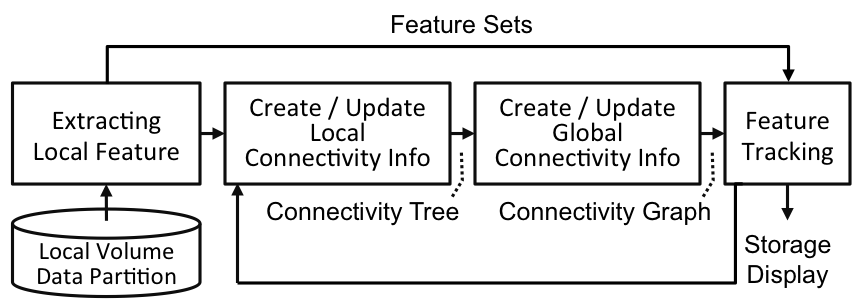
\includegraphics[width=1.0\linewidth]{workflow.png}
\caption{The major steps of our parallel feature extraction and tracking process.}
\label{fig:workflow}
\end{figure}

It is challenging to extract and track features of large time-varying volume data in parallel. First, although a feature can be extracted partially on a processor using the conventional methods, we need to build the connectivity information of the feature across multiple processors. Such information allows us to obtain the global description of a feature from a set of neighboring processors, and enables more advanced operations such as statistical analysis and feature similarity evaluation. Second, such connectivity information can be dynamically changed with features evolving over time. We need to update and maintain the connectivity of features in an efficient fashion to track highly intermittent phenomena.

However, building and maintaining connectivity information of features typically require intensive data exchanges among processors, and thus incurs extra communication cost. To address this issue, we adopt the master-slave paradigm~\cite{Chen03realtime}, but carefully design our parallel feature representation and schedule inter-processor communication to prevent the host from becoming the bottleneck. The local connectivity information is computed and preserved only by the slaves where the correspondent features reside. Hence, there is no global connectivity information maintained at the host. The host only serves as an interface to broadcast the criterion of features to the slaves. In this way, the computation of merging local information is distributed to the slaves. Thus, we can effectively reduce the potential communication bottleneck on the host.

In addition, our approach does not need to set a barrier to wait for all connectivity information to be sent back to the host. Thus, if there exists the features that span over a large number of nodes but are not explored by a user, the potentially long computation time for these features will not block the whole process. This makes it ideal for an interactive system, where users can select the features of interest and instantly receive the visual feedback as the features evolve.

Without loss of generality, for each time step, we partition the volume data into a regular grid of blocks. We then distribute the data blocks among processors, and each processor is assigned with one block.\footnote{Our method can be easily extended to the case that each processor is assigned with multiple data blocks.} In general, a feature can be any interesting object, structure or pattern that is considered relevant for investigation. Here, a feature is defined as the collection of voxels enclosed by a certain iso-surface. Given a sufficiently fine grained partitioning, some features can cross multiple data blocks.

We consider the following two factors in our communication scheme design for better performance and scalability:

\begin{itemize}
	\item $N_{com}$ : The number of communications required to build the connectivity information;
	\item $N_{proc/com}$ : The number of processors involved in each communication.
\end{itemize} 

\subsection{Extracting Partial Local Features}

%------------------------------------------------
\begin{figure}[t]
	\centering
	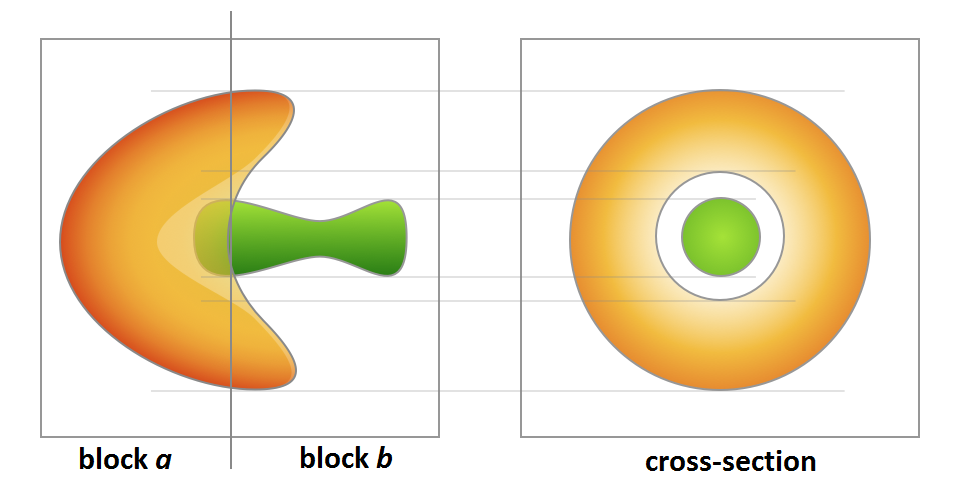
\includegraphics[width=0.9\linewidth]{figure1@2x.png}
	\caption{Two features cross two blocks and share the same centroid on the cross-section.}
	\label{fig:special}
\end{figure}
%------------------------------------------------

Volume features can be extracted using conventional techniques such as region growing, geometry or topology based clustering, or other domain specific algorithms. In this work, we use a standard region-growing algorithm\cite{Lohmann1998} to identify partial features in each data block. This is done by first spreading a set of seeding points inside each data block, and then grow the voxels into a set of separate regions, each regarded as a single feature. As the data is distributed, a feature can cross multiple blocks, and each processor is not aware of the partial features identified on the other processors in this stage. 

\subsection{Matching Partial Local Features}

For the features across multiple blocks, their cross-sections in both sides of the adjacent blocks should match. Therefore, we can connect two partial features by comparing their cross-sections on the corresponding boundary surfaces. That is, two adjacent processors can find the possible matches of the partial features through exchanging and comparing their boundary voxels. Using a ghost area that stores the boundary surface belonging to a neighbor may help to achieve voxel-wise matching for the partial features. However, maintaining such ghost areas requires frequent inter-process communication and is considerably expensive for interactive applications. 

To reduce communication cost and accelerate comparison, we use a simplified method to detect matches. We first represent the cross-section on a boundary surface as:

\begin{itemize}
	\item $P_{centroid}$: The geometric centroid of the cross-section of the feature;
	\item $P_{min}$ and $P_{max}$: The minimal and maximal coordinates of the cross-section area.
\end{itemize}

%------------------------------------------------
\begin{algorithm}[t]
\caption{Match of two partial features $f$ and $f^{'}$}
	\begin{algorithmic}
		\IF{$abs(P_{centroid} - P_{centroid}^{'}) \leq 1$ 
		\textbf{and} $abs(P_{min} - P_{min}^{'}) \leq 1$ 
		\textbf{and} $abs(P_{max} - P_{max}^{'}) \leq 1$}
			\STATE return $f$ \textbf{matches} $f^{'}$
		\ENDIF
	\end{algorithmic}
\label{alg:match}
\end{algorithm}
%------------------------------------------------

For two partial features, we then compare their geometric centroids. If the difference is larger than 1-voxel offset, we consider that they belong to different features. However, only considering geometric centroids is not sufficient to match two features. In some special cases, two different features can have the same geometric centroid on the boundary surface, as shown in Figure~\ref{fig:special}. Therefore, we also need to consider the min-max coordinates of the cross-section areas to detect bipartite matching of partial features, as shown in Algorithm~\ref{alg:match}. In this way, we only need to exchange 3 coordinate values, which, in most cases, are sufficient to detect feature connection across a boundary in practice.

\subsection{Creating Local Connectivity Tree}

Based on our method to match the partial local features, we can abstract the local connectivity information using a tree structure. As shown in Figure~\ref{fig:match}. each data block has six direct neighbors (the outermost blocks have less), each with a shared boundary surface. The connectivity tree is constructed by taking the block as root and its six adjacent blocks as its first level child nodes. A leaf is appended to a first level node if and only if a local feature touches the corresponding boundary surface. Note that a feature can touch multiple boundary surfaces and thus be attached to multiple first level nodes.

Each voxel in the local data block has a unique global index, and thus each leaf can be encoded using 3 integers (global index for $P_{centroid}$, $P_{min}$ and $P_{max}$). We use $P_{centroid}$ as the feature index, and sort the sibling leaves according to the indexes in ascending order. In addition, the root and the first level child nodes can be encoded with the indexes of corresponding data blocks, which are irrelevant to the number of features-on-boundary (henceforth referred as $N_{fb}$). Therefore, the overall spatial complexity of a local connectivity tree for each data block is $\theta(3*N_{fb})$, which is typically negligible compared with the volume size. 

%------------------------------------------------
\begin{figure}[t]
	\centering
	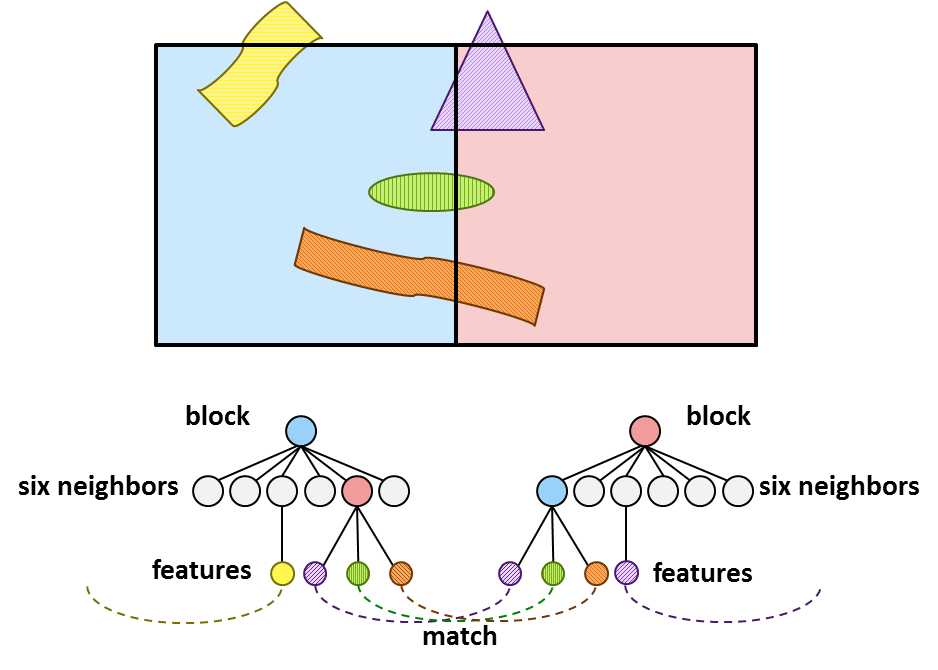
\includegraphics[width=1\linewidth]{match.png}
	\caption{Top: Two blocks with four features across the blocks. Bottom: The tree structure used for maintaining local connectivity information, where the root node is encoded with the block index, its child nodes are encoded with the indexes of its neighboring blocks, and the leaves of each first level child node represent the local partial features. The leaves should match the ones residing on the corespondent neighboring block, which are indicated by the dashed lines.}
	\label{fig:match}
\end{figure}
%------------------------------------------------

From the perspective of temporal complexity, the creation of a local connectivity tree does not introduce an extra computational cost as it can be done along with the region growing process. The values of $P_{centroid}$, $P_{min}$ and $P_{max}$ are updated only if a feature reaches the boundary surface.

\subsection{Creating Global Connectivity Information}

After a local connectivity tree is created within each data block, their leaves need to be exchanged and merged to obtain the overall description of a partitioned feature. The exchanging and merging process is decisive in that its effectiveness largely affects the overall performance and scalability of the feature tracking algorithm as a whole.

\subsubsection{Representation of Connectivity Information}

Based on the tree structure of the local connectivity information, the global connectivity information can be described as a graph that connects the local connectivity trees, as shown in Figure~\ref{fig:match}. To facilitate data exchanges among processors, we adopt the linear representation techniques~\cite{AMET1990} and represent the global connectivity information into a feature table. Each feature has a global unique ID. The table is indexed by the feature IDs, and each entry lists the processors that contains the corresponding partial local features. Given this simple representation, once a user selects a feature, each related processor can query the table to identify the other processors that need to be communicated to collectively operate on the selected feature.

\subsubsection{The Centralized Approach}

One possible solution to build the global feature table is to directly use the master-slave paradigm. When the feature extraction process is done, all local connectivity trees are gathered to the host processor. Then the host starts to merge the leaves from each connectivity tree and matches the partial features to build the global feature table.

The merit of this centralized approach lies in that it requires inter-processor communication only once; that is, $N_{com} = 1$ for each processor. Moreover, the global feature table can be preserved in the host that it can directly respond to feature queries without collecting information from the slaves again. However, this approach has an obvious drawback. Since all local connectivity trees are sent to the host, the number of processors involved in each communication is $N_{proc/com} = N_p$, and there exists potential contention, both in communication and computation, on the host.

\subsubsection{The Decentralized Approach}
\label{sec:decentralized}

A better solution is to decentralize the gathering and merging process from using a single host processor to exploiting all available processors. After the feature extraction process is done and so does the creation of local connectivity tree, an \emph{all-gather} process starts to exchange all local connectivity trees among processors. Each processor first collects a full copy of all local trees and merges the leaves to obtain the global feature table. However, this approach does not actually resolve the contention problem since every processor acts like the host and it still needs to gather and merge all local trees. 

%------------------------------------------------
\begin{figure}[t]
	\centering
	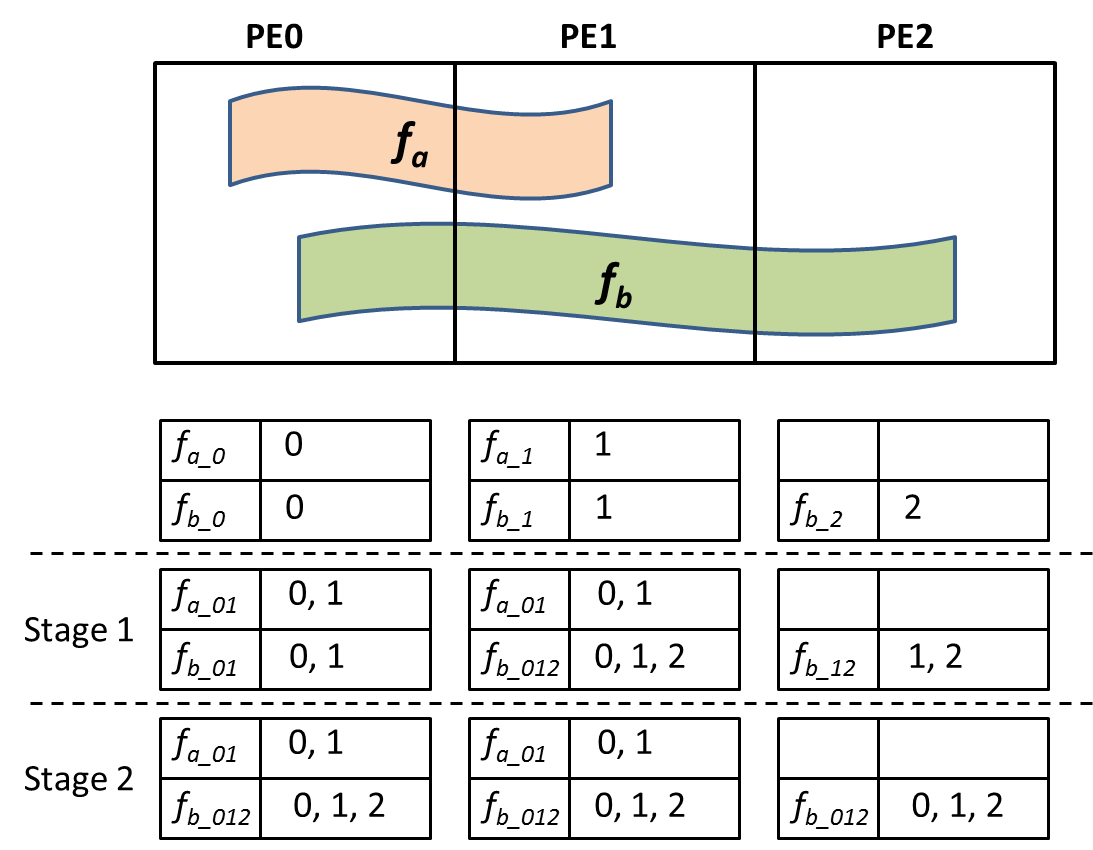
\includegraphics[width=0.9\linewidth]{global_feature_table.png}
	\caption{Construction of partial global feature table with three processors and two features. There are two communication stages. At each stage, each processor only communicates with its immediate neighbors. Each entry of the table is indexed by the feature IDs and lists the processors that contain the corresponding feature.}
	\label{fig:global_table}
\end{figure}
%------------------------------------------------

We observe that, for a real-world data set, it is rarely the case that all features are spanning over every data block. In addition, it is unnecessary for each processor to construct a global feature table to contain all features. Each processor only needs to construct a partial table that records the other processors sharing the same set of features. Thus, it is possible for a processor to communicate with a small set of processors to construct the needed portion of the table. However, on the other hand, we also observe that each processor has no information of the partial features identified on the other processors. Thus, initially, a processor is not aware of other processors with which can be directly communicated to gather the partial features. 

Based on these observations, we design an iterative approach that uses a multi-stage communication scheme. During each stage, each processor only communicates with its immediate neighbors to exchange and propagate the feature connectivity information. This could be considered as a higher level of region growing process that starts from one seeding block and grows to adjacent blocks by exchanging and merging connectivity information in a breadth-first fashion, until all cross-boundary features are connected. 

Figure~\ref{fig:global_table} gives an example of the procedure to construct a partial global feature table with three processors and two features.\footnote{For simplicity, we use an example of 1D partitioning. However, the procedure can be easily extended to 3D cases.} We can see that the feature $f_a$ is identified by the processors PE0 and PE1, and the feature $f_b$ is identified by PE0, PE1 and PE2. Initially, each processor constructs a partial global feature table initialized with only the local features with their local IDs, such as $f_{a\_0}$, $f_{b\_2}$, and so on. In the first stage, PE0 exchanges the local connectivity tree with PE1, and PE1 exchanges the tree with PE2. After exchanging trees, each processor independently matches the partial features, and updates the corresponding feature IDs and entries in its table. For example, the ID of $f_a$ has been changed to $f_{a\_01}$ on both PE0 and PE1, and the entry contains the same processor list. However, for $f_b$, as the information has not been propagated between PE0 and PE2, its ID is different on the three processors. In the second stage, each processor still only communicates with its immediate neighbors, and the information of $f_b$ has been propagated to PE0 and PE2 through PE1. Thus, for $f_b$ ID and its processor list are all the same on the three processors. After an extra communication, each processor detects there is no further information sent from its neighbors, and thus the construction of the partial global feature table is completed.

After constructing its partial global connectivity table, for any selected features, each processor can easily find other corresponding processors. For example, in Figure~\ref{fig:global_table}, if $f_a$ is selected, PE0 and PE1 can mutually find that each other belongs to the same communicator, while PE2 is excluded.

The reason we choose the six-direct-neighbor paradigm is because it can minimize the communication cost. It takes a maximum of ${3n-1}$ times communications, where $n$ denotes the maximum processor number among the axes. This corresponds to the maximum communications needed for propagating the information of a feature that covers the whole domain, although this case is nearly impossible in practice. The temporal complexity for garnering all necessary leaves is hence as low as ${O(\sqrt[3]{N_{proc}})}$. And the number of processors involved in each communication is a constant of a maximum of six, i.e., $N_{proc/com} \leq 6$.

Another optional paradigm is to let each processor communicate with its 26 neighbors, including the adjacent diagonal blocks. Communication with the adjacent diagonal block takes as much as half the time for any block to reach its furthest diagonal. However, $N_{proc/com}$  is also increased to 26. For data sets where features only span over a small number of blocks, the 6-direct-neighbor paradigm outweighs the 26-neighbors paradigm in communication complexity.

\subsection{Updating Global Connectivity Information}

%------------------------------------------------
\begin{figure}[t]
	\centering
	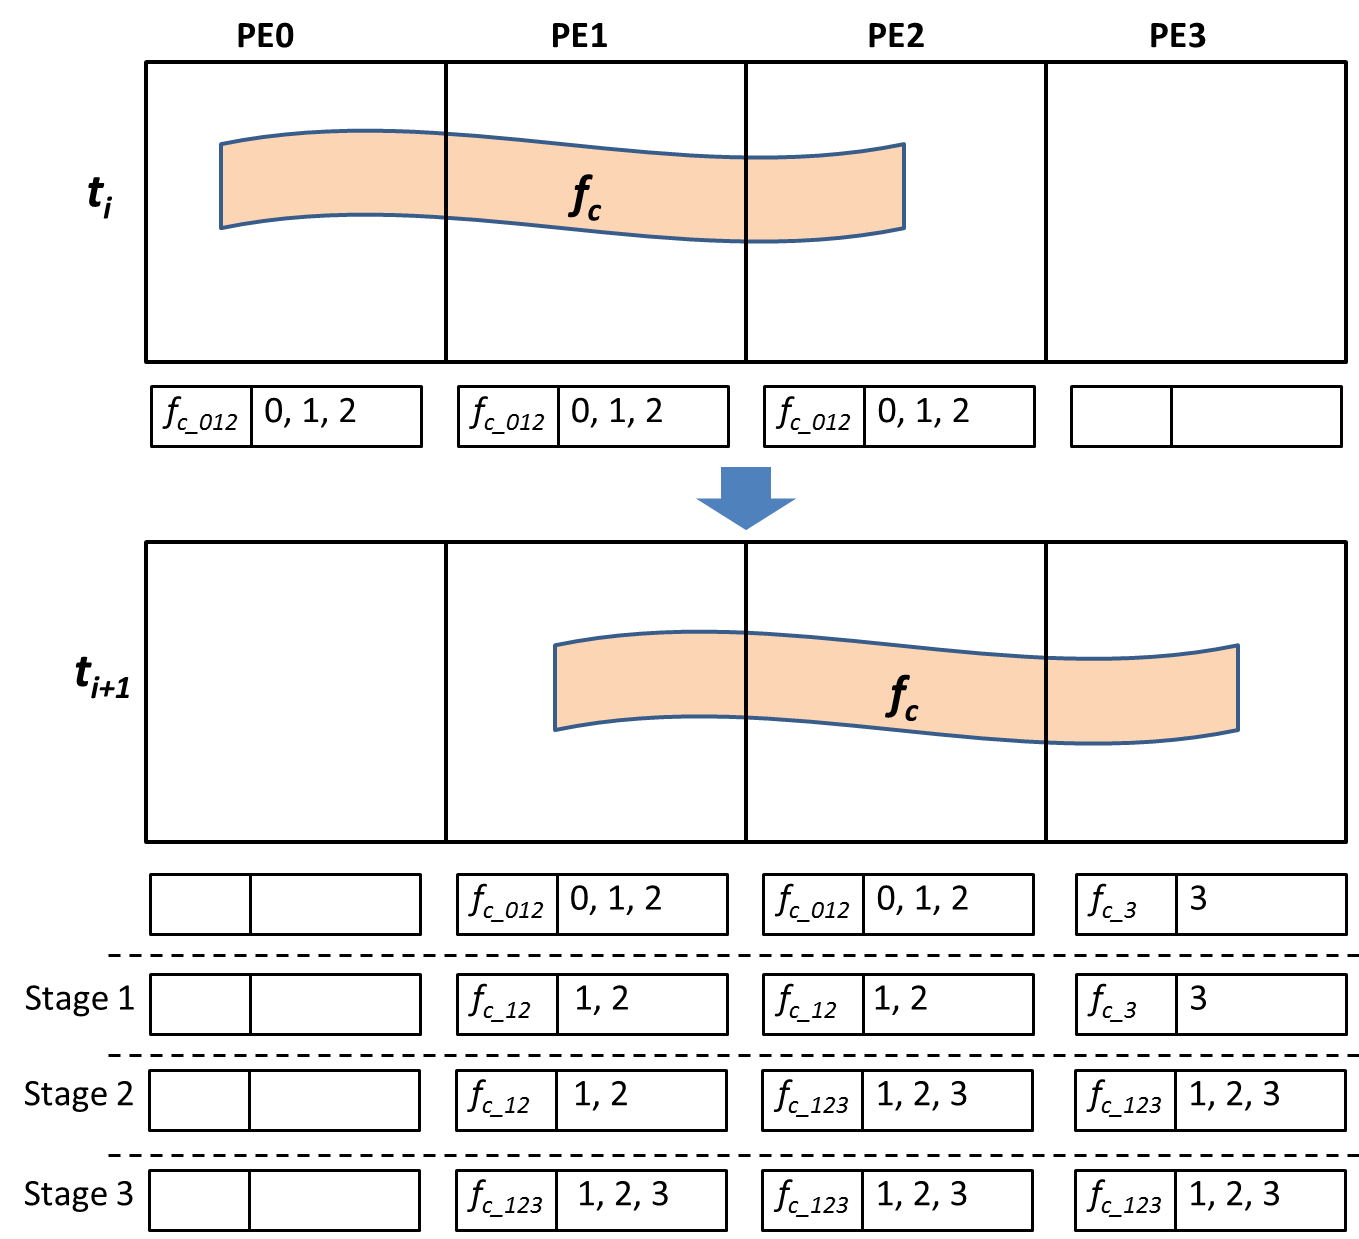
\includegraphics[width=1\linewidth]{global_grow_feature_table.png}
	\caption{Update of partial global feature table with four processors and one feature. Feature $f_c$ is extracted and adjusted in Stage 0 followed by three communication stages to record the possible shrinking and expanding of the feature. }
	\label{fig:hybrid}
\end{figure}
%------------------------------------------------

To track features, we can construct the global connectivity table for each time step. However, if the time interval is sufficiently small for generating the data, volumetric features may drift but should not change drastically in neither size, shape, nor location. We assume that the changes of each feature are within the range of one block. Based on this assumption, we can optimize feature tracking by incrementally updating the global connectivity information over time.

As depicted in Figure~\ref{fig:hybrid}, each processor constructs a partial global feature table at time step $t_i$. Meanwhile, we maintain a communicator, $\textbf{C}$, which contains the corresponding processors for each feature. For example, feature $f_c$ spans over PE0, PE1, and PE2. These three processors have the same table entry with respect to $f_c$. The table of PE3 is empty at $t_i$. PE0, PE1 and PE2 belong to the same communicator $\textbf{C}$.

For the next time steps, $t_{i+1}$, each processor continues to predict and correct boundaries as to extract partial local features. For the existing features, their IDs are retained in the partial global feature table. For the new features, their IDs are added into the table. And the IDs are erased from the table if the corresponding features drift away from that block. As shown in Figure~\ref{fig:hybrid}, $f_c$ leaves PE0 and enters PE3. In this case, the table of PE0 becomes empty, and the table of PE3 adds a new entry. At this time point, the feature ID on PE3 is not the same as the others, as the feature has not been matched yet. In addition, PE0, PE1 and PE2 still belong to $\textbf{C}$. 

Then we start to update the connectivity information. In the first stage, PE0, PE1, and PE2 perform an \emph{all-gather} operation within their communicator $\textbf{C}$ to update the connectivity. PE0 is then removed from the corresponding entry on PE1 and PE2, and also removed from $\textbf{C}$. In the second stage, each processor exchanges the local connectivity information with the immediate neighbors as the decentralized approach in Section~\ref{sec:decentralized}. The information of $f_c$ is propagated between PE2 and PE3. In the third stage, all the processors in the communicator $\textbf{C}$ perform an \emph{all-gather} operation again to update the connectivity. The information of $f_c$ is propagated to the rest of processors $\textbf{C}$, and then PE1, PE2, and PE3 have the same table at $t_{i+1}$. Given the unified information, we can then update the communicator $\textbf{C}$ by including PE3 with respect to $f_c$. 

This update procedure can be easily extended to the circumstances with more processors and features. We note that the cost of collective communication is marginal within a communicator of limited size. By leveraging this nice property, for each feature, we only need at most three stages to update the connectivity information, independent of the length of the feature.